%% This is an example first chapter.  You should put chapter/appendix that you
%% write into a separate file, and add a line \include{yourfilename} to
%% main.tex, where `yourfilename.tex' is the name of the chapter/appendix file.
%% You can process specific files by typing their names in at the 
%% \files=
%% prompt when you run the file main.tex through LaTeX.
%% prompt when you run the file main.tex through LaTeX.
\chapter{Use of a Global Model to Understand Speciated Atmospheric Mercury Observations at Monitoring Sites in Latin America }
%% BACKGROUND
\begin{flushleft}
Environmental pollution from Hg can damage ecosystems through its transformation into toxic methylmercury and bio-accumulation in food chains. Further, Hg is highly mobile in the atmosphere, allowing it to travel to faraway places, resulting in worldwide distribution of its elemental form, \hg, which can last for as long as six months in the atmosphere\cite{horowitz_new_2017,shah_improved_2021}. Hg in the atmosphere can be classified as gaseous elemental Hg (GEM), gaseous oxidized Hg (GOM), and particulate-bound Hg (PBM) less than 2.5$\mu$m in diameter \cite{lindberg_synthesis_2007,schroeder_atmospheric_1998,landis_development_2002}. In most cases, Hg emissions occur as gaseous elemental Hg0, which is relatively inert and sparingly soluble in water\cite{horowitz_new_2017}. Since most Hg entering ecosystems comes from the atmosphere, monitoring and modeling atmospheric Hg and Hg deposition enables us to understand its biogeochemical cycle. In addition, a better understanding of Hg's circulation in the environment would enable effective policies to reduce its harmful effects.
\end{flushleft}
\section{Background}
\begin{flushleft}

According to Brasseur and Jacob, (2017), it is crucial to have a large ensemble of observations to evaluate atmospheric Hg modeling outputs, and several studies have published results using different ensembles of Hg monitoring data. Until now, no detailed model comparison has been conducted in some world regions with high anthropogenic Hg emissions, such as Latin America. Studies analyzing modeling results in these regions have been limited due to a lack of high-frequency atmospheric Hg monitoring capacity in these regions, as illustrated in Figure \ref{fig:global-hg-monitoring-networks}, which illustrates the distribution of global Hg monitoring networks published in the GMA 2018. As seen in Figure \ref{fig:global-hg-monitoring-networks}, Latin America, Africa, and South East Asia remain significantly behind Europe and North America regarding access to relevant observation ensembles. 
\end{flushleft}

\begin{figure}[H]
  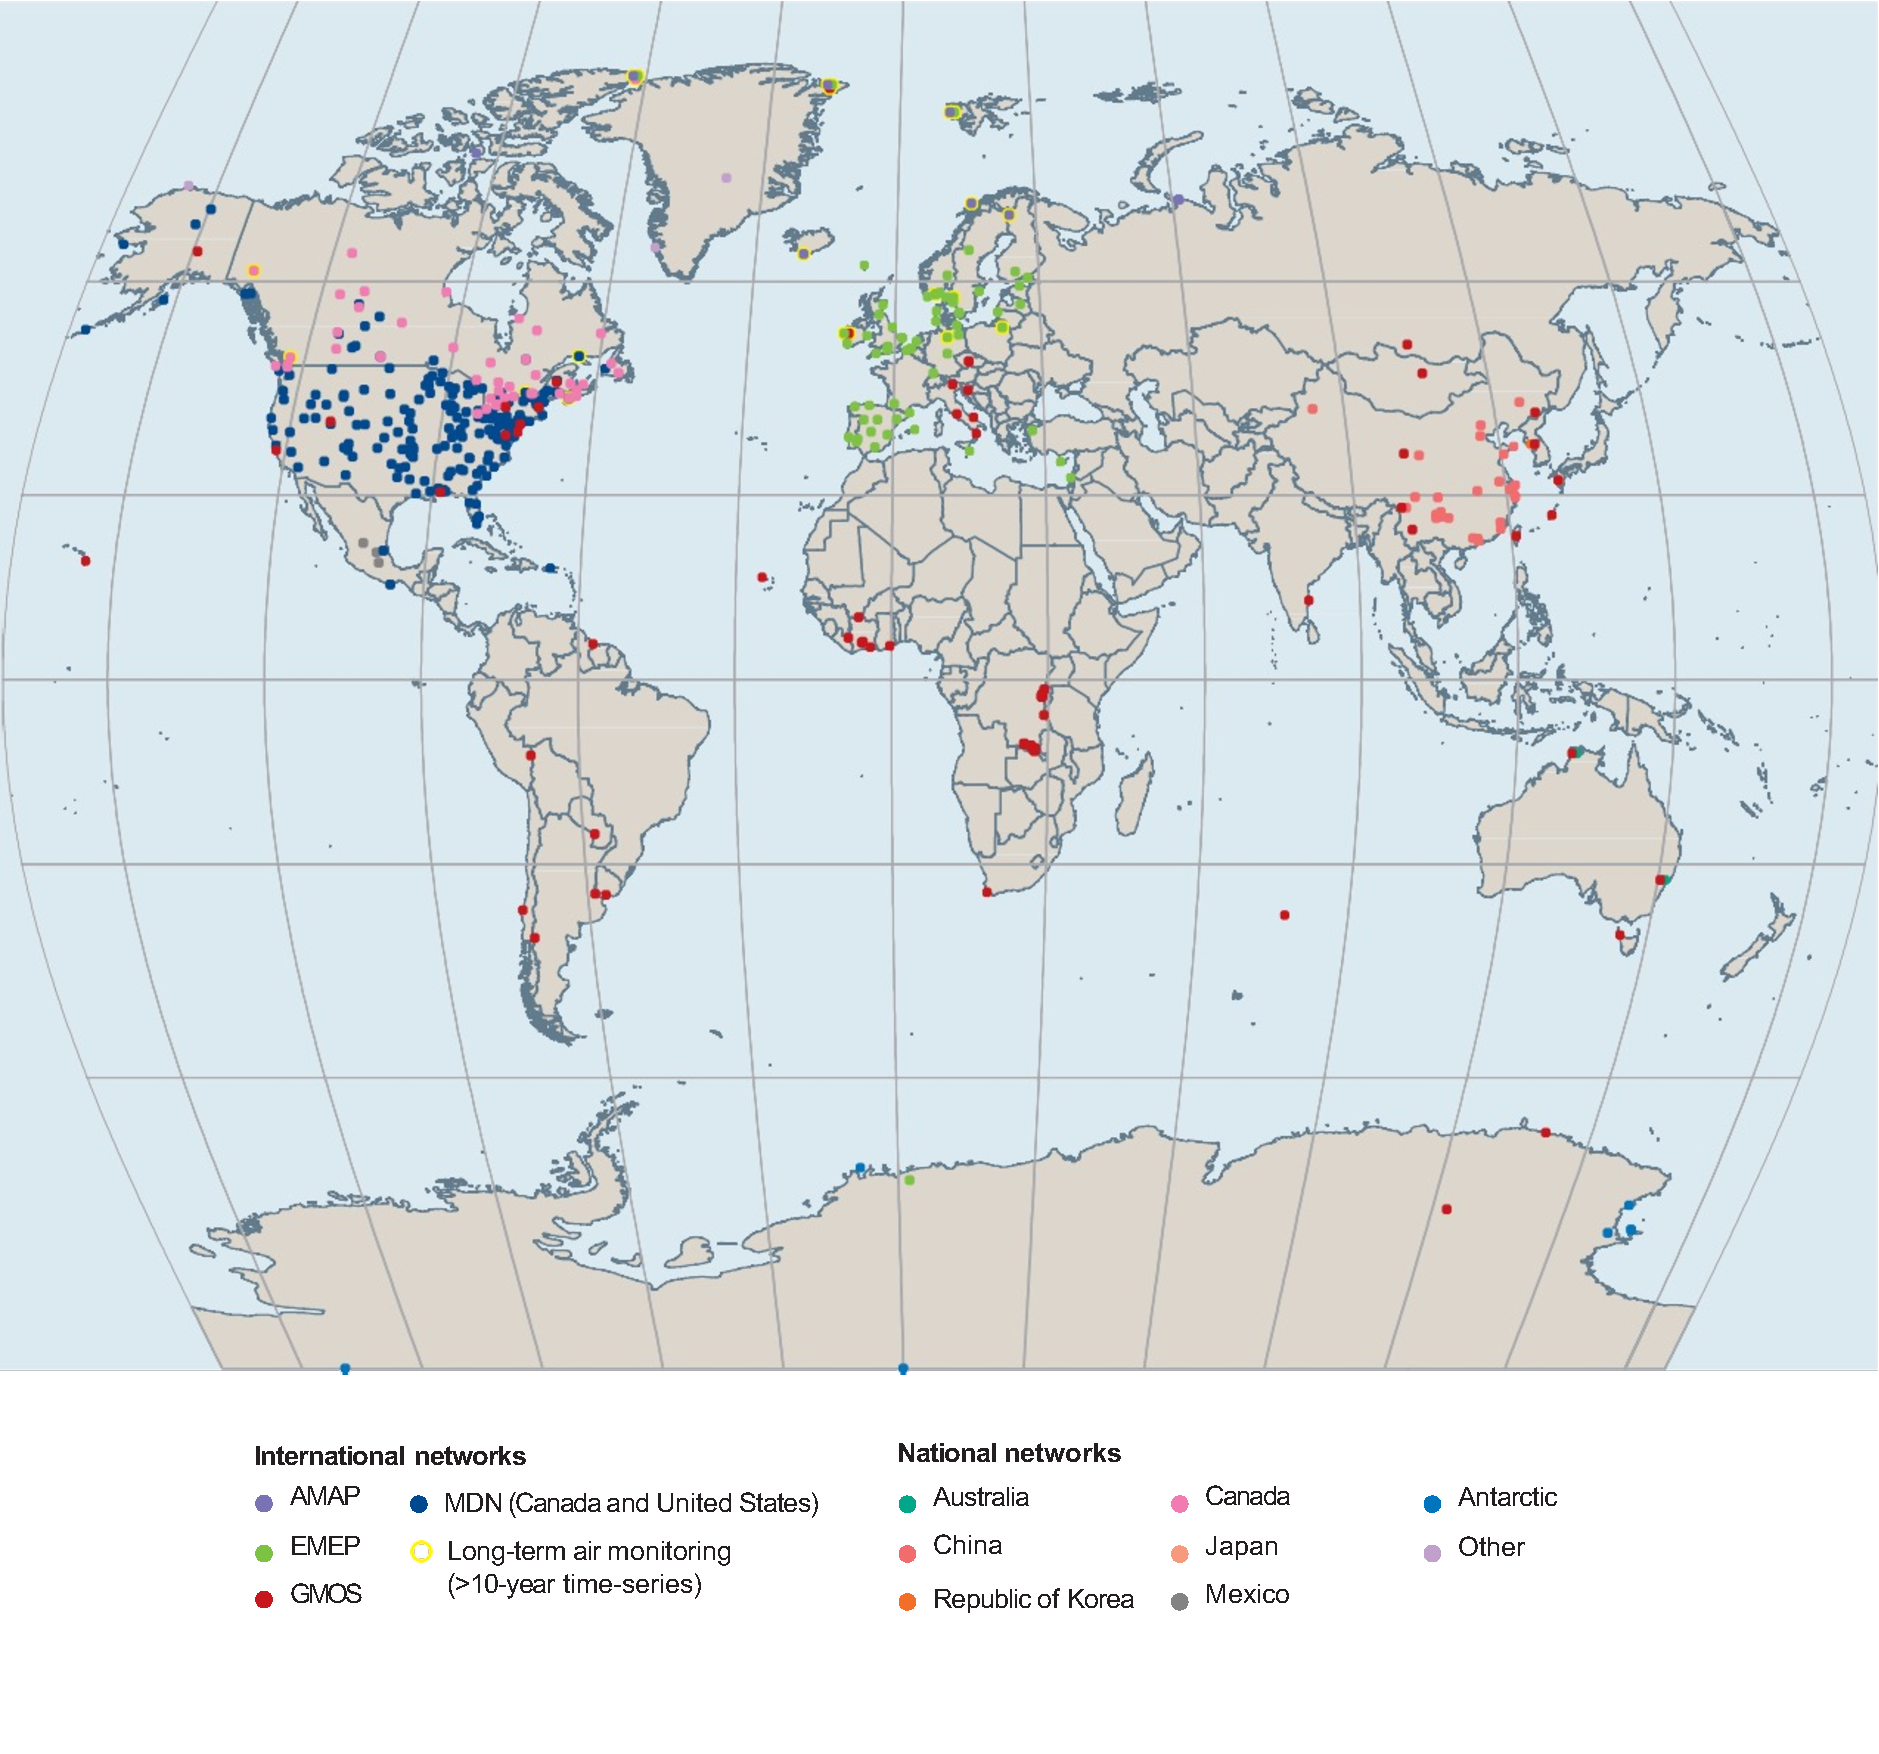
\includegraphics[width=\textwidth]{templates/figures/global-hg-monitoring-networks.pdf}
  \caption{Global map of Hg monitoring networks \cite{united_nations_environment_programme_technical_2019}}
  \label{fig:global-hg-monitoring-networks}
  \centering
  
\end{figure}
\FloatBarrier

\begin{flushleft}
 In this chapter, I employ the GEOS-Chem model with observed Hg at multiple sites in Latin America. I combine simulations of Hg in the atmosphere produced by the \gc CTM (Sect. 2.2.1) with ground-based observations of atmospheric total gaseous mercury (TGM) (Sect. 2.2.2) from the Global Mercury Observation System (GMOS)\cite{sprovieri_atmospheric_2016} and gaseous elemental mercury (GEM) data from a network of passive air samplers (PAS) distributed across Latin America. Section 2.3 presents results and discussion\cite{quant_measuring_2021}. Comparisons of observations and model outputs are given in Sect. 2.3.1. Finally, I discuss the implications of the current state of atmospheric monitoring and modeling atmospheric Hg in Latin America (Sect. 2.3.2) and summarize my conclusions (Sect. 2.4).
\end{flushleft}




%%----------------------------METHODS-------------------------------------------
\section{Methods}
\subsection{GEOS-Chem Description}
\begin{flushleft}


Global atmospheric Hg concentration was simulated using version 12.8.1 of GEOS-Chem, whose Hg simulation is described by Horowitz et al. (2017)\cite{horowitz_new_2017}. All the simulations in this study were run globally for 47 vertical layers at a resolution of 2.0$\times$2.5, which is approximately equal to a 222 km$\times$277.5 km grid square at the equator \cite{horowitz_new_2017}. Moreover, the MERRA-2 assimilated meteorological data,\cite{gelaro_modern-era_2017} drive the model's atmospheric transport, which calculates atmospheric Hg from three tracers: elemental Hg, Hg\textsuperscript{0}, divalent Hg, Hg\textsuperscript{2+}, and particulate-bound divalent Hg,Hg\textsuperscript{p}. The Hg chemical scheme in the GEOS-Chem version used in this study considers bromine (Br) to be the primary \hg oxidant\cite{horowitz_new_2017} and employs monthly mean Br oxidant concentrations from Schmidt et al.,(2016)\cite{schmidt_modeling_2016}. 
\end{flushleft}
\begin{flushleft}
\subsection{GEOS-Chem Simulations}
The GMA 2018 emissions inventory was used to represent anthropogenic emissions sources from all sectors\cite{steenhuisen_development_2019}. Different inputs to the GEOS-Chem model, such as emissions sources, can be toggled on or off depending on the research objective; hence a reference simulation, \on was created by turning on all Hg emissions sources globally. Moreover, a \off was generated by turning off the ASGM source globally to evaluate the contribution of ASGM to the baseline \hg in the atmosphere by calculating the difference between the \on and \off.
\end{flushleft}


\begin{table}[H]
\captionof{table}{Description of GEOS-Chem Simulations Conducted}
\label{tab:geos_chem_simulation_description}

\centering
\resizebox{\textwidth}{!}{\begin{tabular}{lcp{0.6\linewidth}}

Simulation Name  & Resolution & Description  \\
                        
\hline
Base (ASGM=ON)         & 2.0$\times$2.5 & All Hg anthropogenic emission sources are turned on  \\
No ASGM (ASGM=OFF)        & 2.0$\times$2.5 & All ASGM emissions are turned off

\end{tabular}}

\end{table}
\begin{flushleft}
 The frequency of the simulation output was set to output daily \hg averages at the global scale, while the \hg output for the grid boxes corresponding to the locations of the GMOS observation sites was set to an hourly frequency. The GEOS-Chem outputs for all the simulations conducted were in units of parts per trillion (ppt) and were converted to \nang at standard temperature and pressure (273 K, 1 atm) to compare them to observations.
\end{flushleft}

\subsection{Observation Data}
\begin{figure}[H]
 \centering
  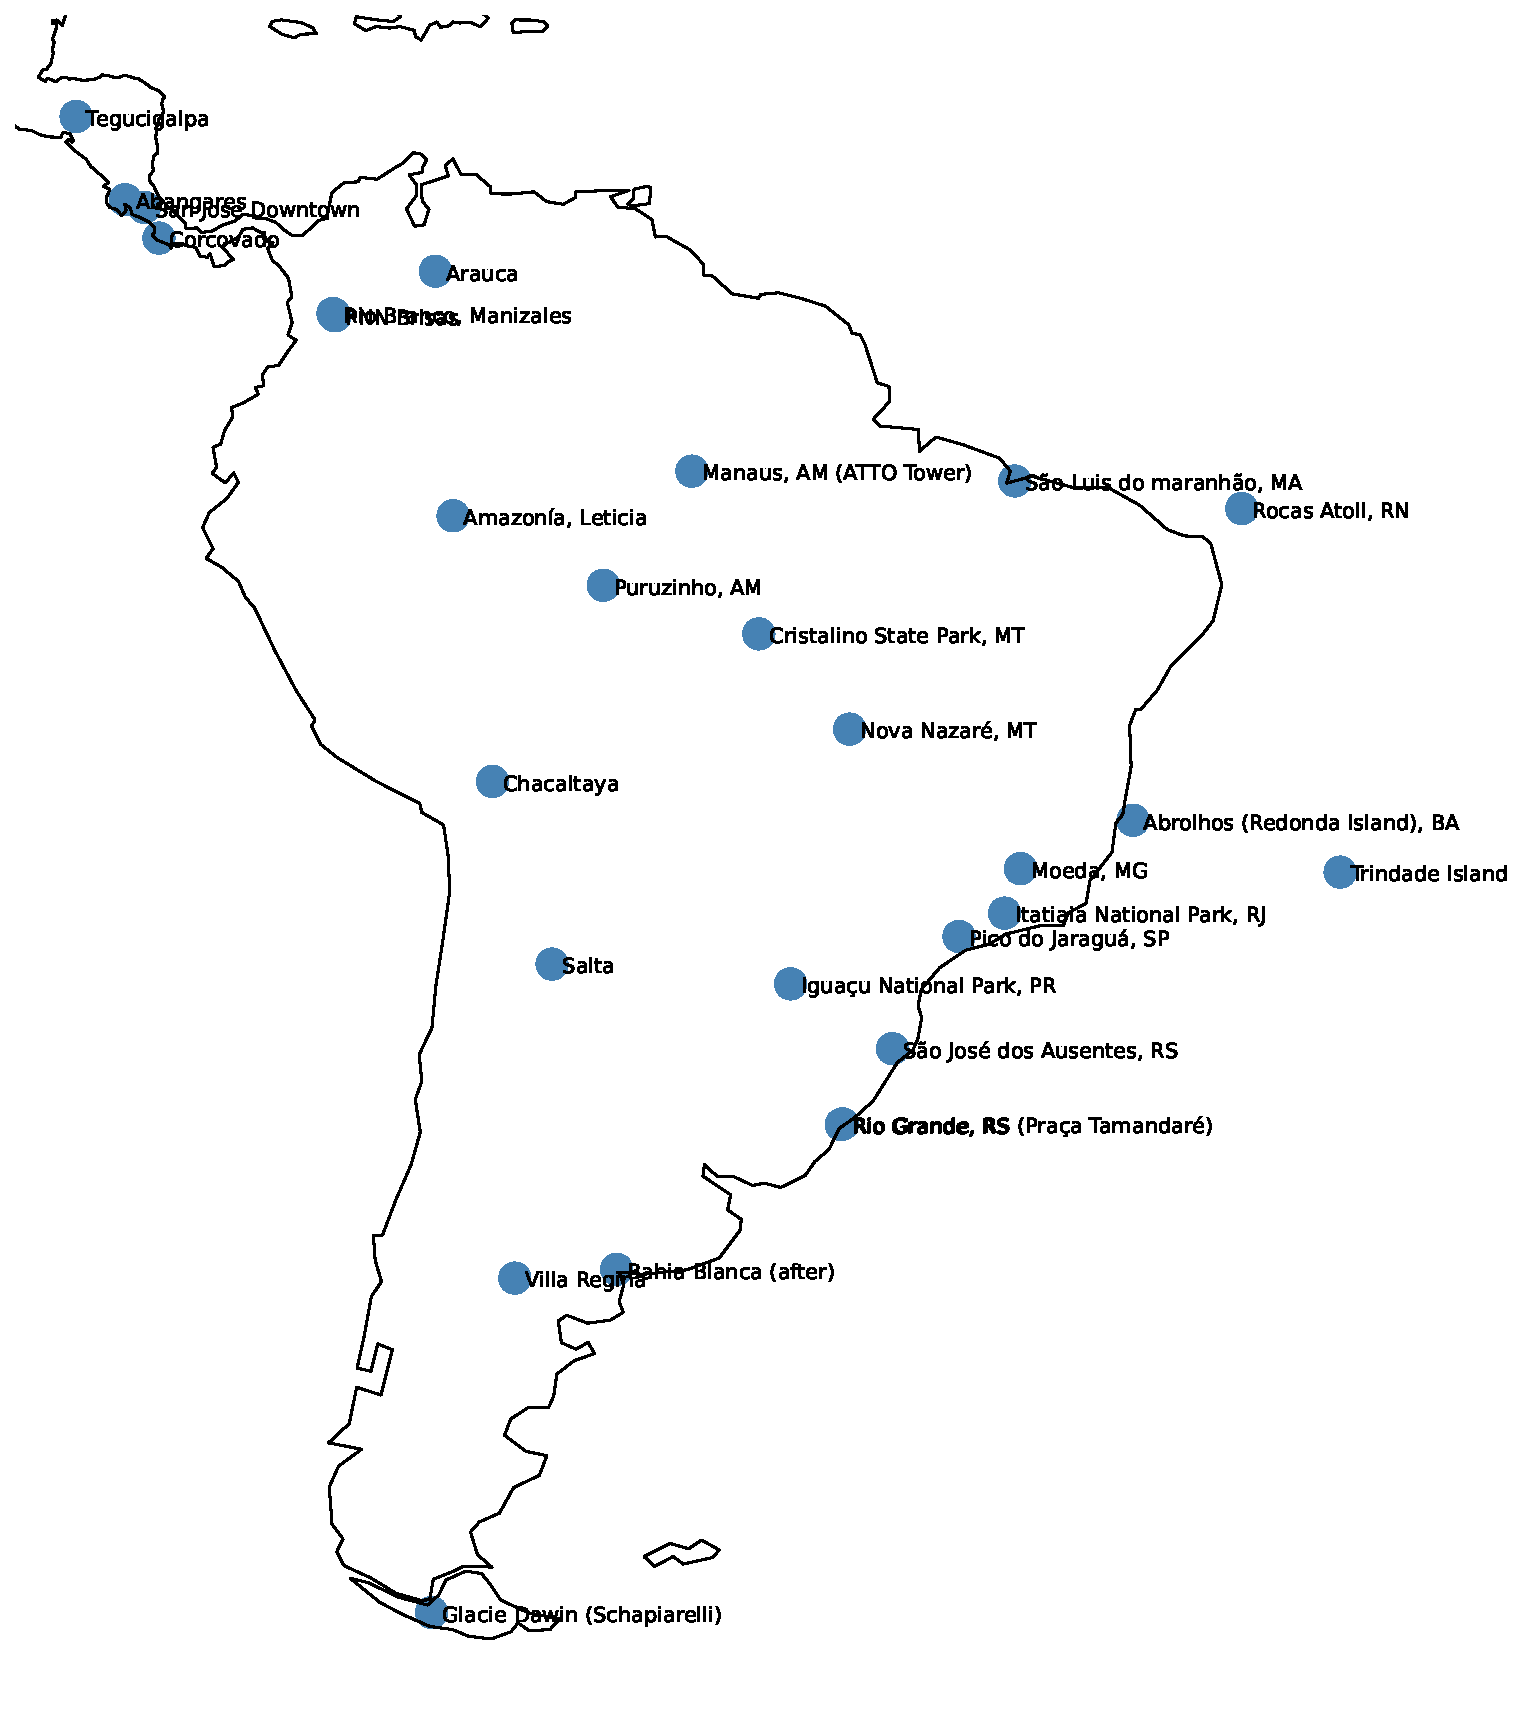
\includegraphics[width=0.8\textwidth]{templates/figures/Passive_Samplers/Latam_Passive_SamplerSites.pdf}
  \caption{Map Showing the GMOS Monitoring Network Sites and Passive Sampler Locations in South America \cite{quant_measuring_2021,koenig_seasonal_2021}}
  \label{fig:GMOS_PAS_stations_map}
 
  
\end{figure}
\FloatBarrier

\begin{flushleft}
 GMOS is one of a few major global projects to develop a global observing system for mercury pollution. A vast network of ground-based monitoring stations, regular oceanographic cruises, and lower, upper, and stratospheric measurements make up this European-funded project \cite{sprovieri_atmospheric_2016,koenig_seasonal_2021}. More than 40 ground-based monitoring sites constitute the international network, covering many regions with limited to no observational data available before GMOS\cite{sprovieri_atmospheric_2016}. The GMOS monitoring network sites in Latin America are shown by the circles with a red outline on Figure \ref{fig:GMOS_PAS_stations_map}. Available Hg observation data from the GMOS stations on Figure  \ref{fig:GMOS_PAS_stations_map} was obtained from the GMOS online database (http://www.gmos.eu), as well as published studies about the Hg monitoring data from the different sites  \cite{koenig_seasonal_2021}. Additionally, average annual GEM concentration data for 27 sites in Latin America was obtained from Quant et al. (2021), which included information about the coordinates of the deployment sites and the period of measurement \cite{quant_measuring_2021}. These measurements were carried out by passive air samplers (PAS),  and the respective locations of the PAS are shown by the blue circles in Figure \ref{fig:GMOS_PAS_stations_map}. In contrast to active Hg monitoring equipment such as those used in the GMOS network, which can be prohibitively expensive, energy-intensive, and require extensive training, PAS require no energy to operate and do not require any special handling skills. Furthermore, PAS can be easily deployed for long periods. This combination of attributes of PAS allows more sampling sites to be studied over extended periods enabling significant average GEM concentration estimates to be obtained. 
\end{flushleft}




\subsection{ Observation Data Manipulation}
\begin{flushleft}
The hourly measurements of total gaseous mercury (TGM) in the atmosphere in \nang retrieved from the online GMOS database were converted to daily averages and compared to the GEOS-Chem modeled \hg concentration at the various sites for the period between 2012 and 2016.  The PAS data was compared to the annual average Hg concentration for 2015, and the coordinate information from the PAS data was used to directly compare the GEM observations and model outputs at the respective PAS sites.
\end{flushleft}
\begin{table}[H]
\captionof{table}{The comparison of the model predictions of the average Hg concentration for the available measurement period}
\label{tab:ASGM_at_GMOS_annual_avs}

\centering
\resizebox{0.5\textwidth}{!}{\begin{tabular}{lcl}
  \hline

GMOS  & Number of Records &  Measurement Period \\
\hline
Sisal           &   320 & 1/1/2010-1/1/2016 \\
Calhau          &   309 & 1/1/2013-12/1/2014 \\
Niew Nickerie   &   215 & 3/1/2007-12/1/2014 \\
Manaus          &   100 & 1/1/2013-12/1/2014 \\
Chalcataya      &   333 & 7/1/2014-2/1/2016 \\
  \hline
\end{tabular}}

\end{table}

%%----------------------------RESULTS AND DISCUSSION---------------------------
\section{Results and Discussion}
\subsection{GMOS Observations vs GEOS-Chem}
\begin{figure}[H]
\centering
  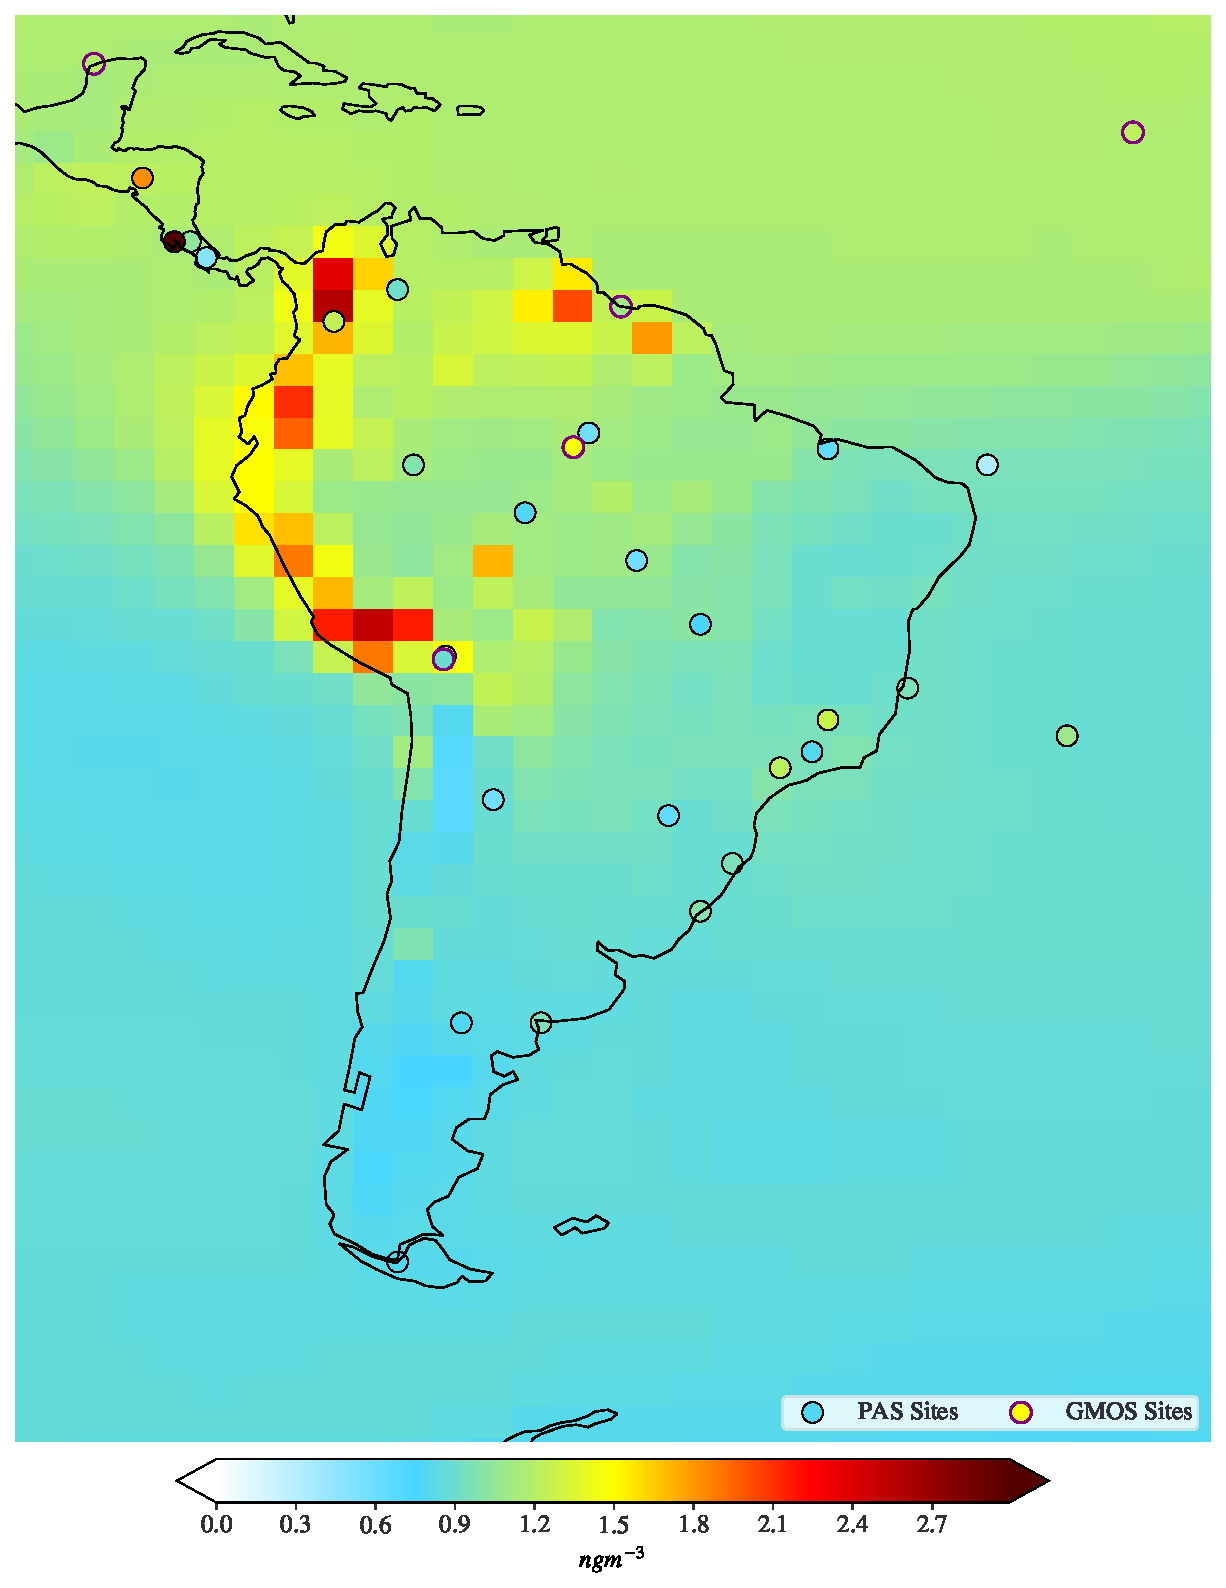
\includegraphics[width=0.7\textwidth]{templates/figures/Passive_Samplers/07-27-22_pas_vs_model_Hg0-per-year_001.pdf}
  \caption{Annual average Hg concentration on the surface in Latin America averaged. The background is the annual average \hgc produced by the \on for 2015. The circles with the black outline are the annual average GEM concentration from the PAS sites, while the circles with the purple outline are the annual average TGM concentrations from the GMOS sites.}
  \label{fig:06-12-22_pas_vs_model_Hg0-per-year_001}
  
  
\end{figure}
\FloatBarrier
\begin{flushleft}
A striking trend in most plots of the observed vs modeled Hg concentration on Figure \ref{fig:GMOSvsGC} is the GEOS-Chem model's general overestimation of the Hg concentration and mismatch in the variability. The observed average daily TGM concentration at the GMOS sites (red line) is compared to the modeled \on average daily \hg (blue line) and the ASGM contribution (black line). The different Hg concentrations were plotted as a function of time-based on the availability of data records between 2012 and 2016. None of the sites had a continuous data set that spanned the entire period of interest, but the Niew Nickerie and Manaus sites had the most minor data records at 215 days and 100 days, respectively, as seen in Table \ref{tab:ASGM_at_GMOS_annual_avs}.   
\end{flushleft}
% \begin{table}[H]
% \captionof{table}{The comparison of the model predictions of the average Hg concentration for the available measurement period}
% \label{tab:ASGM_at_GMOS_annual_avs}

% \centering
% \resizebox{\textwidth}{!}{\begin{tabular}{lcccccc}
%   \hline

% GMOS & Observed Hg\textsuperscript{0} & Observation Standard & Base(ASGM=ON) Hg\textsuperscript{0} & Base(ASGM=ON) Standard  & ASGM Contribution  Hg\textsuperscript{0}   \\
% Sit & (ng m$^{-3}$)/year             & Deviation ($\sigma$) & (ng m$^{-3}$)/year                   & Deviation ($\sigma$)      &(ng m$^{-3}$)/year\\
                        
% \hline
% Sisal           &   1.19    & 0.14 & 1.27 & 0.05 & 0.12  \\
% Calhau          &   1.22    & 0.12 & 1.30 & 0.04 & 0.11  \\
% Niew Nickerie   &   1.11    & 0.23 & 1.41 & 0.06 & 0.25  \\
% Manaus          &   1.49    & 0.31 & 1.27 & 0.09 & 0.23  \\
% Chalcataya      &   0.90    & 0.16 & 1.20 & 0.14 & 0.28  \\
%   \hline
% \end{tabular}}

% \end{table}
\begin{figure}[H]
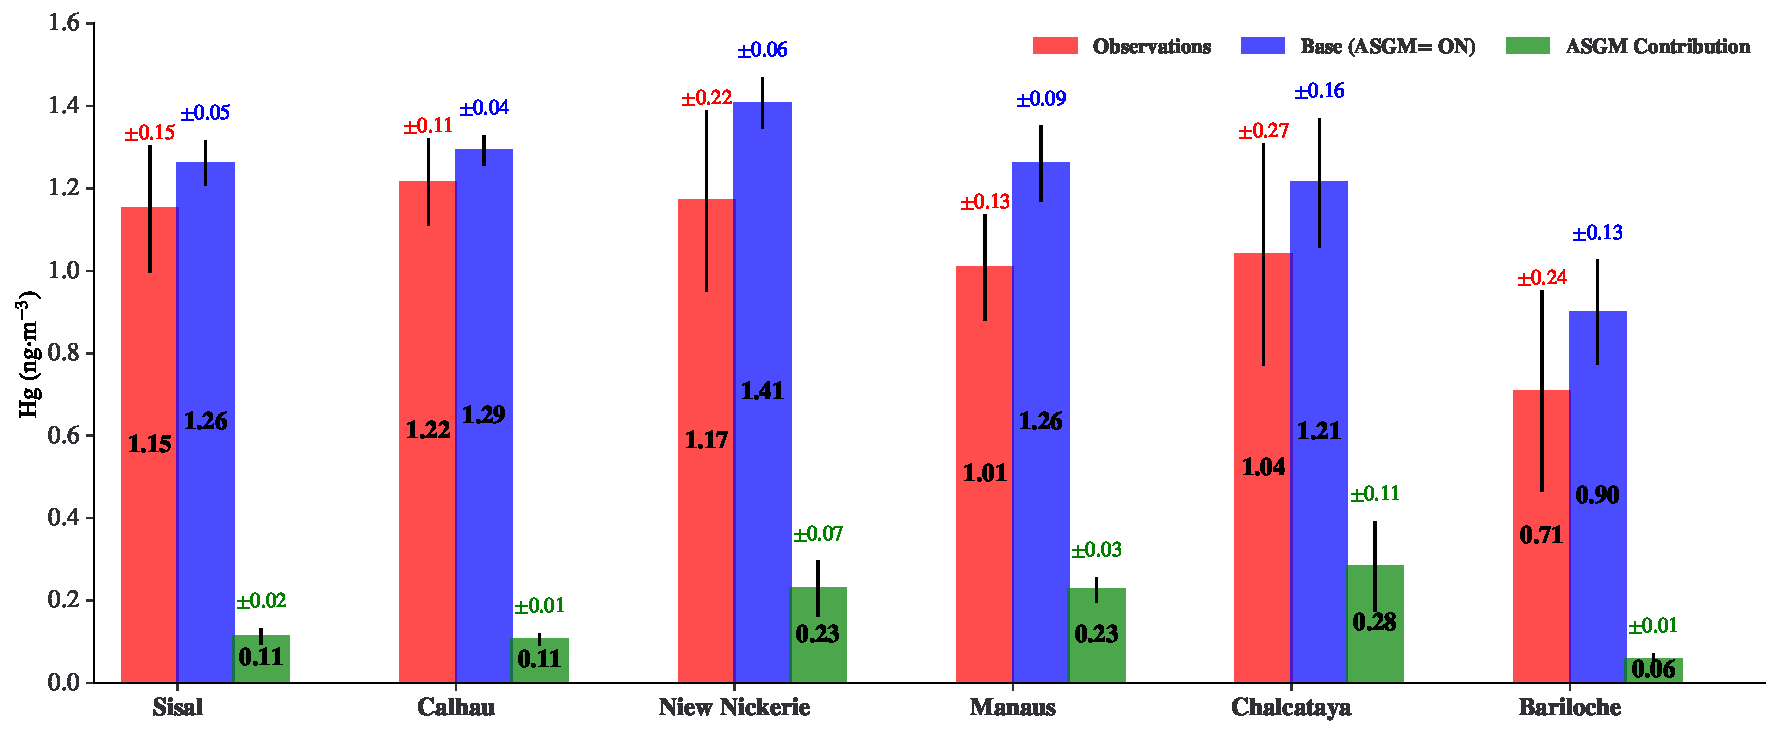
\includegraphics[width=\textwidth]{templates/figures/GMOS_Sites/gmos_sites_stats.pdf}
\centering
\captionof{figure}{Time series plots of the observed TGM concentrations at different GMOS sites in red with the corresponding modeled concentration in blue and the associated ASGM contribution in black. Available observations and corresponding model output between January 2013 and January 2015 were plotted except for the CHC site, whose data is from July 2014 and January 2016}
\label{fig:GMOSvsGC}
\end{figure}
\FloatBarrier


\begin{flushleft}
Another significant aspect of the model observation comparison on Figure \ref{fig:GMOSvsGC} is the low predicted ASGM contribution at  four of the GMOS sites in contrast to the variability that closely matches the observed variability at the Chalcataya (CHC) site. A plausible explanation of models predicted ASGM contribution to the \hg at the GMOS location might be attributed to the CHC site's proximity to the Madre de Dios region in Peru, a known source of enormous ASGM Hg emissions. 
\end{flushleft}

\begin{figure}[H]
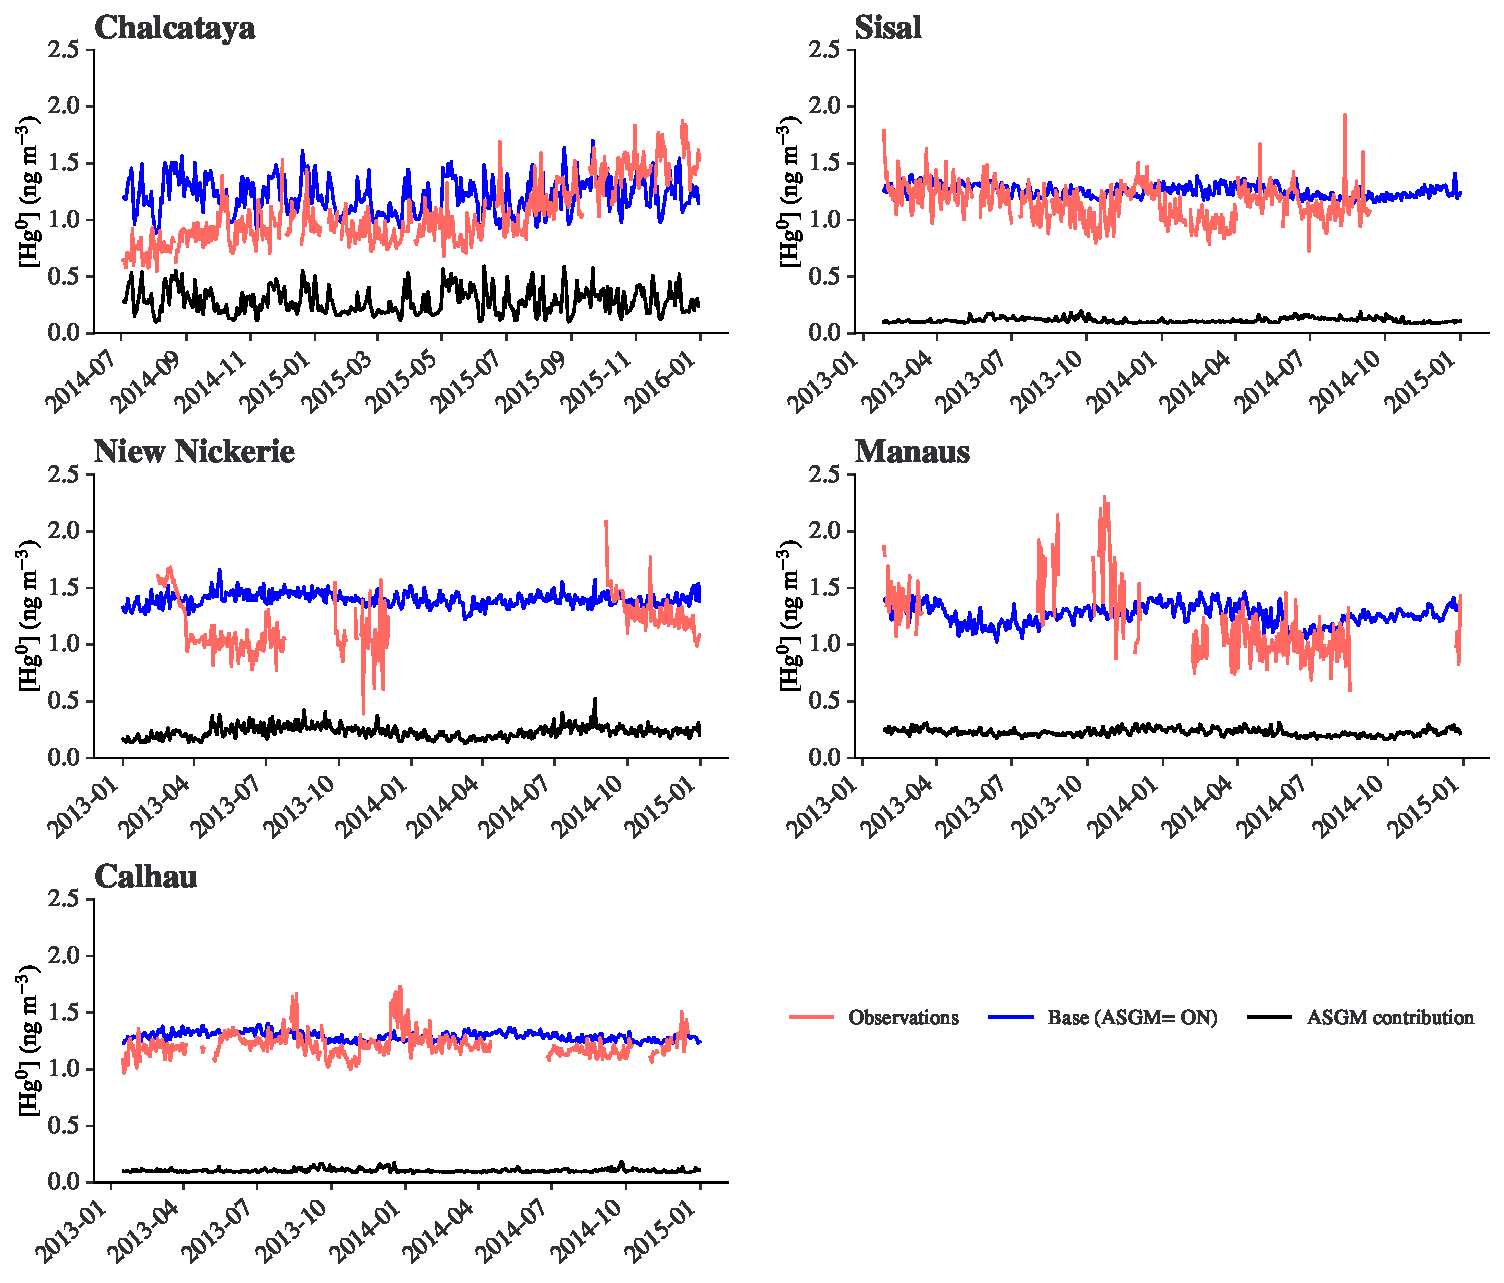
\includegraphics[width=\textwidth]{templates/figures/GMOS_Sites/GMOS_Sites.pdf}
\centering
\captionof{figure}{Time series plots of the observed TGM concentrations at different GMOS sites in red with the corresponding modeled concentration in blue and the associated ASGM contribution in black. Available observations and corresponding model output between January 2013 and January 2015 were plotted except for the CHC site, whose data is from July 2014 and January 2016}
\label{fig:GMOSvsGC}
\end{figure}
\FloatBarrier

\begin{flushleft}
Moreover, the Niew Nickerie and Manaus sites had the worst mean and variability relationship with the modelled \hg as seen on Table \ref{tab:modelvsobs metrics}. Even though the GEOS-Chem model overestimates the mean concentration over a one-year period of measurement except for the Manaus site, as seen in Table \ref{tab:ASGM_at_GMOS_annual_avs}, the estimates for the mean concentration at Sisal and Calhau are within a 10\% margin as shown in Table \ref{tab:modelvsobs metrics}. The model's deficiency in predicting the mean may result from the model's poor parameterization of processes such as dry deposition and wet deposition. Poor parameterizations of ASGM Hg emissions in the model may also  contribute to the poor model skill in predicting the mean. Furthermore, the time series plot of the Hg concentrations at CHC shows a general upward trend that is not represented in the other observations and the model. 
\end{flushleft}


\begin{flushleft}
  
\end{flushleft}

\begin{table}[H]
\captionof{table}{Table showing the extent to which the model predicts the observations showed by the percentage difference between the model predictions and the observations }
\label{tab:modelvsobs metrics}

\centering
\resizebox{0.5\textwidth}{!}{\begin{tabular}{lcc}
  \hline

GMOS  &Percentage difference & Percentage difference  \\
Site & annual mean (\%) & standard deviation (\%)           \\
                        
\hline
Sisal           & 6.72  &-64.29  \\
Calhau          & 6.56  &-66.66   \\
Niew Nickerie   & 27.03 &-73.91    \\
Manaus          & -14.77&-70.97    \\
Chalcataya      & 33.33 &-12.5   \\
  \hline
\end{tabular}}

\end{table}
\begin{flushleft}
 
\end{flushleft}


% \subsection{Passive Sampler Observations vs GEOS-Chem}
\begin{flushleft}
 The comparison between the modeled concentration in the atmosphere and the PAS data corroborated the finding that the GEOS-Chem model overestimated the observed concentrations in the atmosphere, as seen in Figure \ref{fig:06-12-22_pas_vs_model_Hg0-per-year_by-latitude_001} which shows the modeled (blue circles) and observed (red circles) annual average \hg plotted as a function of latitude. The observation error bars represent the replicate precision of the observations, while the model error bars represent the 95\textsuperscript{th} bootstrap confidence interval for the mean annual \hg. Moreover, the PAS observations show high variability as you move from South to North, while the model has low variability and an increasing trend.  
\end{flushleft}

\begin{figure}[H]
  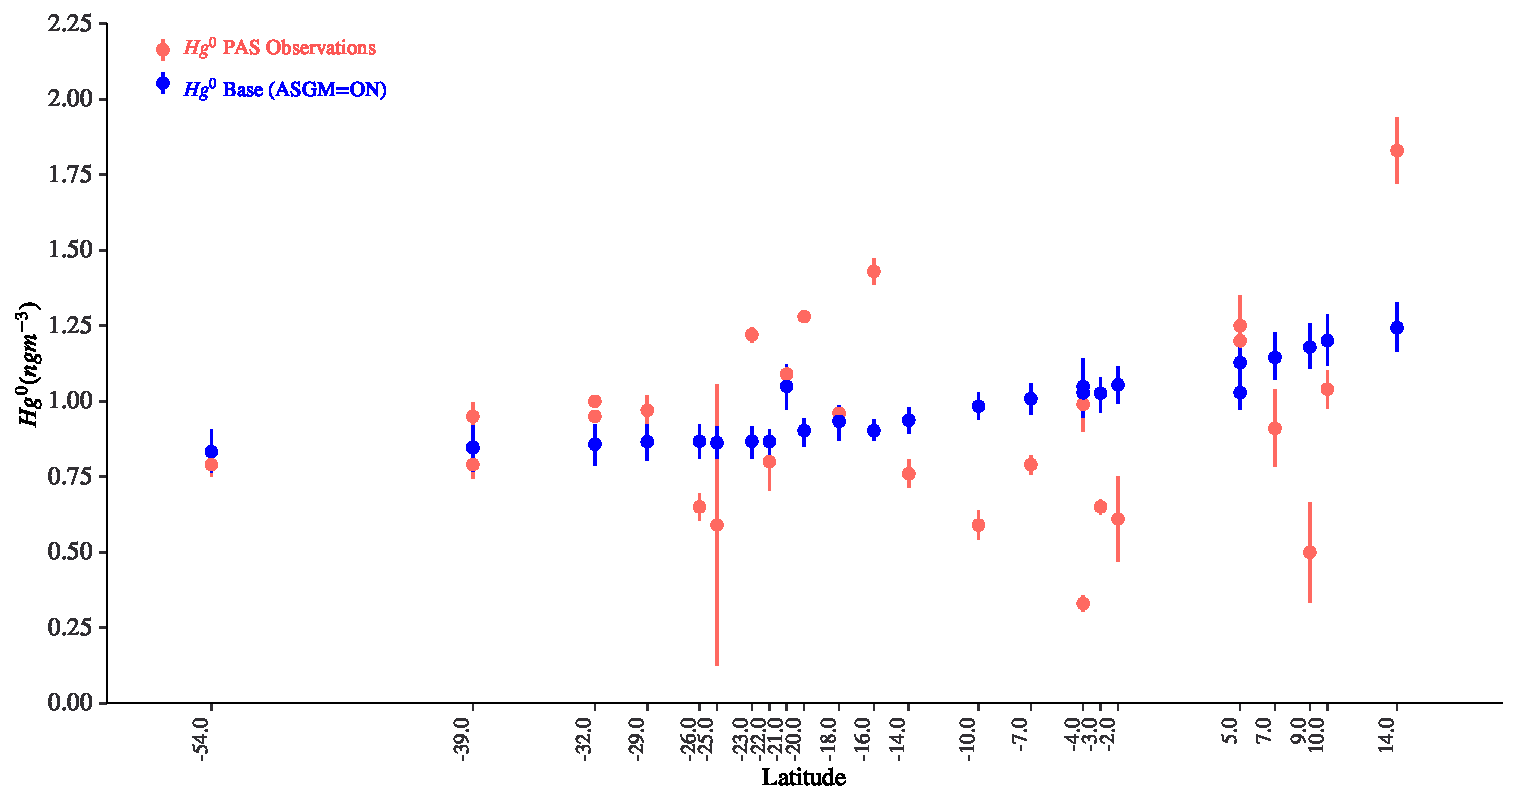
\includegraphics[width=\textwidth]{templates/figures/Passive_Samplers/06-12-22_pas_vs_model_Hg0-per-year_by-latitude_001.pdf}
  \caption{\hg in the atmosphere as a function of Latitude. The \on (blue circles) and observed (red circles) annual average \hg plotted are plotted as a function of latitude to evaluate spatial trends across the continent. The observation error bars represent the replicate precision of the observations while the model error bars represent the 95\textsuperscript{th} bootstrap confidence interval for the mean annual \hg.}
  \label{fig:06-12-22_pas_vs_model_Hg0-per-year_by-latitude_001}
  \centering
  
\end{figure}
\FloatBarrier

\begin{flushleft}
GEOS-Chem's poor predictive capacity observed above is also addressed in Feinberg et al. (2022) where we evaluated atmospheric Hg uptake by vegetation in \gc by constraining vegetation as a Hg sink through a comparison of simulations with a compiled database of litterfall, throughfall and flux tower measurements from 93 forested sites. We found that the \gc version, 12.8  underestimated dry deposition of \hg, which may explain why the observed Hg from the measurements of Hg in the atmosphere at different sites in Latin America was lower than the concentration predicted by the model. Recent studies evaluating the global biogeochemical cycle of Hg argue that Hg concentrations in the atmosphere exhibit an inter-hemispheric gradient from the southern to the northern hemisphere. The annual average \hg modelled by \gc seems to follow the proposed gradient as seen on Figure \ref{fig:06-12-22_pas_vs_model_Hg0-per-year_by-latitude_001}. Furthermore, the PAS measurements, as seen in Figure \ref{fig:06-12-22_pas_vs_model_Hg0-per-year_001} were higher in most of the eastern coastal regions and in the northwestern coastal regions. These high values are the result of the fact that the PASs were placed near populated areas where the Hg background in the atmosphere may also be influenced by Hg emission sources such as power generation and ASGM.

\end{flushleft}











\section{Conclusion}

